\biohead{Kathleen Munday}{Kathleen_Munday}{ }
%\section{Kathleen Munday}\label{Kathleen_Munday}
%\begin{center}
%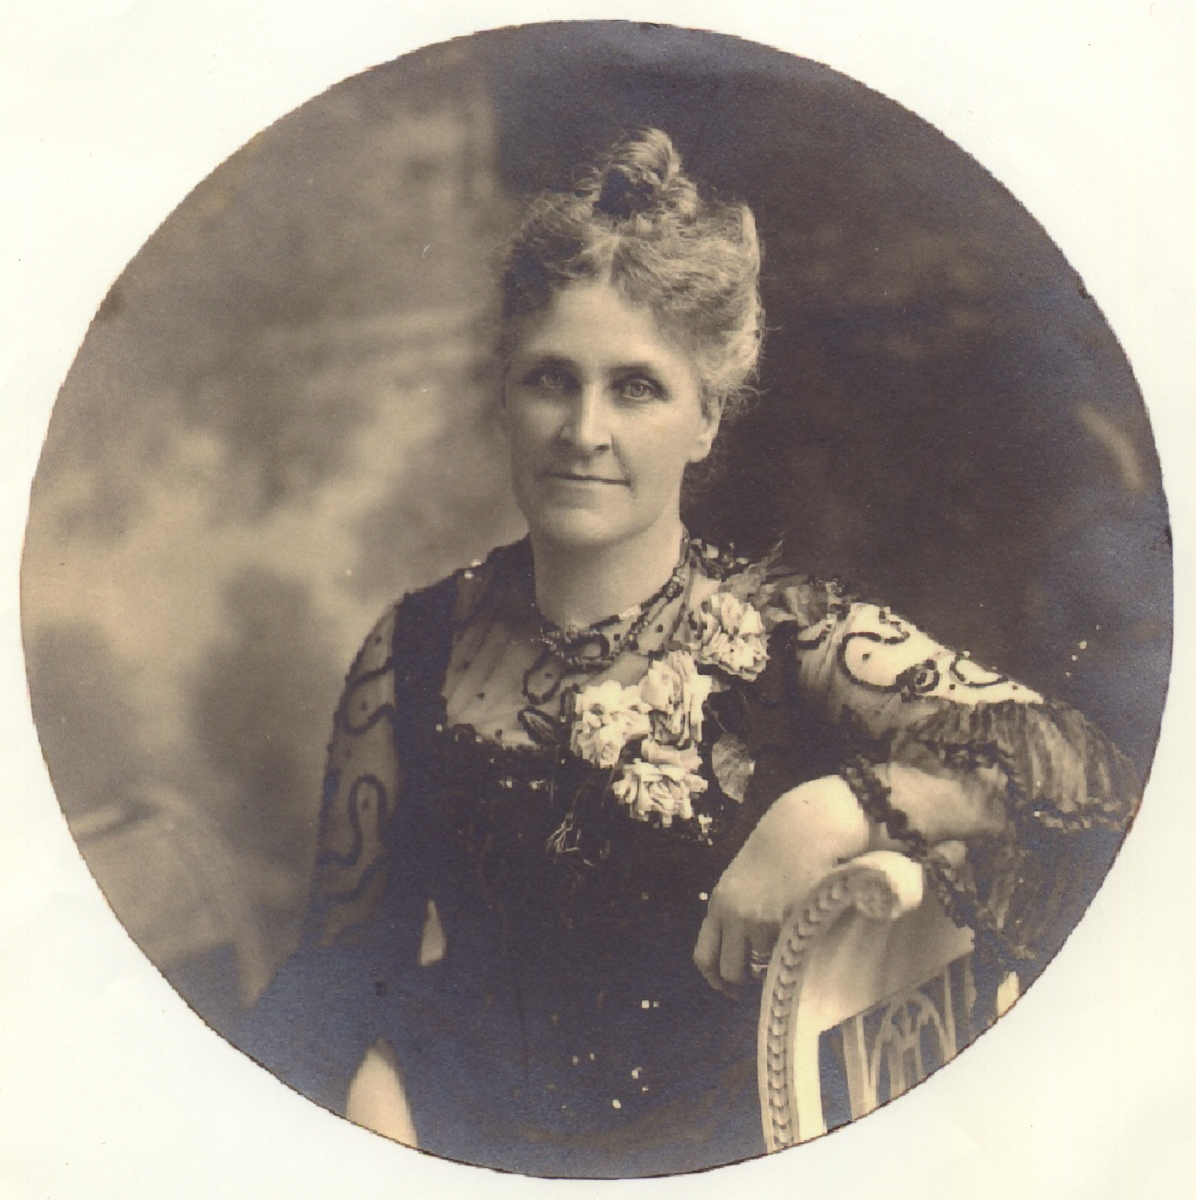
\includegraphics[width=0.8\linewidth]{photos/Kathleen_Munday}
%\end{center}

Kathleen Munday (5 November 1882 -- 17 September 1963) was the second daughter of John Hill Munday (\p{John_Hill_Munday}), who was a partner in a firm of solicitors in London. They lived at The Mendips, Surbiton, Surrey. She was educated at Cheltenham Ladies College, but like most middle class women of her generation did not receive a higher education, nor did she seek employment after finishing school. She was a very accomplished wood carver and artist and received a medal for her fine work. She met James Denton Barker when she was on holiday at Ilkley in Yorkshire and they married just before the outbreak of the first World War, on 4 April 1914. Early the following year their first son, Mead, was born, followed a year and a half later by Ralph (p.\pageref{Ralph_Munday_Denton-Barker}), and then Virginia (p.\pageref{Virginia_Kathleen_Denton_Barker}) in 1919.
